\section{WPA/WPA2}

\subsection{In der Vorlesung wurden mehrere Angriffe auf Basis von Keystream-Reuse für WEP-Verkehre beschrieben (vgl. auch Aufgabe 1). Sind diese auch bei WPA-/WPA2-Verkehren möglich? Begründen sie kurz Ihre Antwort.}
Keystream-Resuse ist nicht mehr möglich, da nun ein Replay-Schutz besteht. Es kann also ein – bspw. durch eine Known-Plaintext Attacke erlangter – Verschlüsselungs-Key nicht wiederverwendet werden, da er bereits verwendet wurde. Außerdem sind die Prüfsummen-Protokolle nicht mehr linear. Dadurch ist auch eine Modifikation einer Nachricht nicht mehr möglich.

\subsection{Welche Angriffe sind heute noch gegen WPA/WPA2 möglich?}
WPA kann mittels Passwortsuche angegriffen werden. Dabei wird eine Schwachstelle des 4-Wege-Handshakes ausgenutzt.
\begin{center}
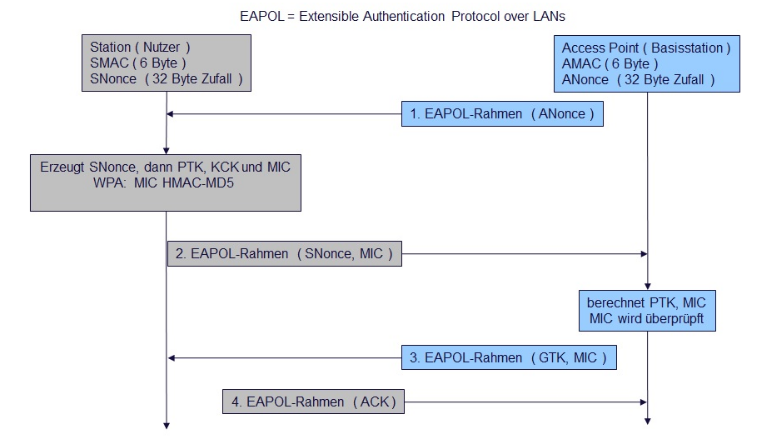
\includegraphics[width=0.8\textwidth]{img/eapol.png}
\end{center}
Zum Zeitpunkt der zweiten Message sind alle Komponenten öffentlich bekannt die für die Erstellung des MIC notwendig sind, außer dem Key Conformation Key (KCK). Dieser leitet sich aus dem Pairwise Transient Key (PTK) ab, dieser wiederum aus dem Pairwise Master Key (PMK), und der wiederum ist der Hash des Passworts mit SSID (der PSK). Somit kann jetzt das Passwort geraten werden. Das Passwort ist dann möglicherweise korrekt geraten, wenn für den abgeleiteten $KCK_i$ gilt:
$$
MIC_{KCK_{i}}(ANonce) \overset{?}{=} MIC_{gesendet}
$$
Hinzu kommt, dass es mittlerweile einen Angriff gibt, der ganz und gar ohne Handshake auskommt. Dabei wird der AP dazu gebracht, einen speziellen EAPOL-Rahmen zu senden, der die PMKID enthält. Dieser ist der Hash von öffentlich übertragenen Werten und dem PMK, wodurch das Passwort so erraten werden kann:
$$
PMKID \overset{?}{=} Hash(Hash(Passwort, SSID), otherPublicStuff)
$$
Bei diesen Angriffen handelt es sich um AP-Spoofing. Diese sind ebenfalls auf WPA2 anwendbar.

\subsection{Wie werden die Angriffe heutzutage, z.B. bei Eduroam, verhindert? Welche Rolle spielen dabei EAP und RADIUS bzw. DIAMETER?}
Mittels EAP wird ein Authentication-Server verwendet. Dieser heißt \textit{RADIUS} (Remote Authentication Dial-In User Service) bzw. \textit{Diameter}. 
\begin{center}
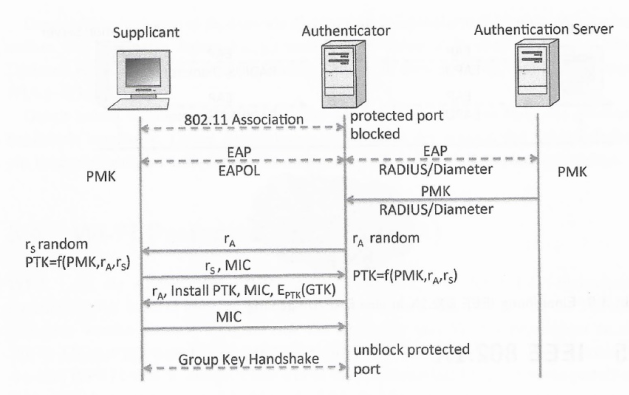
\includegraphics[width=0.8\textwidth]{img/eap.png}
\end{center}
Direkte Verbindungen eines Supplikanten mit dem AP werden direkt von diesem geblockt. Einzig und allein Authentiffizierungs-Anfragen vonseiten des RADIUS werden vom AP angenommen.

\subsection{Was ist die Grundidee des Key Reinstallation Angriffs. Wie kann dieser verhindert werden?}
Grundlage ist das Abfangen des letzten ACKs des Clients, woraufhin dieser nach Verstreich der Frist ein weiteres ACK versendet und der Client macht einen Reset. Jedoch werden die bereits verschlüsselten Daten beibehalten und dort angefangen, wo aufgehört wurde, jedoch mit dem zurückgesetzten Schlüsselstrom. Somit wird eine Reihe von Nachrichten mit demselben Schlüsselstrom verschlüsselt.
$$
c_0 \oplus c_1 = (m_0 \oplus s) \oplus (m_1 \oplus s) = m_0 \oplus m_1
$$
sind nun gewisse $(c_i,m_i)$-Paare bekannt, können diejenigen $m_i$ der dazugehörignen "Equivalenzklasse" entschlüsselt werden. 

Dieser Angriff kann verhindert werden, indem im Protokoll spezifiziert wird, dass der Client nach dem Reset nicht dort weitermacht, wo er aufgehört hat (sondern von vorne), oder dass ggf. gar keine Key-Reinstallation vollzogen wird.

\subsection{Was ist die Grundidee des Krook Angriffs und wie wird dieser durchgeführt. Beschreiben Sie den Angriff beispielhaft.} 
Grundidee ist, dass per Disassoziation der Session Key des Clients zurückgesetzt, genauer auf $0$ gesetzt wird. Der Client aber sendet restliche Pakete mit diesem zurückgesetzten Key, weshalb diese gelesen werden können.
\begin{enumerate}
    \item Oscar schickt eine Deauth-Anfrage an Alice, oder schickt irgendein ungültiges Paket im Namen von Alice an AP-Bob, woraufhin dieser die Deauth-Anfrage an Alice schickt. (Irgendwie sorgt Oscar dafür, dass Alice so eine Anfrage erhält.)
    \item Alice setzt daraufhin ihren Session Key zurück, verarbeitet aber noch die letzten Pakete mit diesem Session Key, wie zu Beginn erläutert.
    \item Oscar fängt die Nachrichten von Alice ab und kann diese nun mitlesen. Sobald Alice wieder angemeldet ist, wiederholt er diese Prozedur.
\end{enumerate}